
\documentclass[11pt]{article}
\usepackage[margin=0.8in]{geometry}
\usepackage{amsmath,amssymb,booktabs,array,longtable}
\usepackage{hyperref}
\usepackage{enumitem}
\usepackage{float}
\usepackage{graphicx} 

\setlist{nosep}

\begin{document}

\begin{center}
{\Large\textbf{Shiv Nadar University Chennai}}\\
\textbf{CS3807 -- Deep Learning Laboratory}\\
\textbf{Experiment 2}\\
{\large\textbf{Implementation of a Multi-Layer Perceptron (MLP) for Multi-Class Image Classification}}
\end{center}

\renewcommand{\arraystretch}{1.25}

\begin{flushleft}
\textbf{Name:} Johan Emmanuel S\\
\textbf{Registration Number:} 24011101043\\
\end{flushleft}

\begin{tabular}{|p{3.8cm}|p{8cm}|p{2cm}|}
\hline
Degree \& Branch & B.Tech Artificial Intelligence \& Data Science & Semester V\\ \hline
Subject Code \& Name & CS3807 -- Deep Learning Laboratory & AY: 2026--27\\ \hline
\end{tabular}

\section{Objective}
To understand the working principle of Convolutional Neural Networks by implementing convolution, pooling, feature map visualization, and image classification using TensorFlow/Keras. 

% Begin Section 2
\section{Learning Outcomes}
Students will be able to: 
\begin{enumerate}
    \item Explain the convolution operation. 
    \item Compute output dimensions using stride and padding. 
    \item Visualize feature maps. 
    \item Implement max pooling and average pooling. 
    \item Calculate CNN parameters. 
    \item Build a CNN for image classification. 
    \item Evaluate CNN performance. 
\end{enumerate}

% Begin Section 3
\section{Background Theory}
A Convolutional Neural Network consists of: 
\begin{itemize}
    \item Convolution Layer 
    \item Activation Layer 
    \item Pooling Layer 
    \item Fully Connected Layer 
\end{itemize}

% Define convolution equation
The convolution operation is: 
\begin{equation}
    Y(i,j) = \sum_{m}\sum_{n}X(i+m,j+n)K(m,n)
\end{equation}
where 
\begin{itemize}
    \item X: Input Image 
    \item K: Kernel (Filter) 
    \item Y: Feature Map 
\end{itemize}

% Define output size equation
The output feature map size is: 
\begin{equation}
    \frac{N-F+2P}{S}+1
\end{equation}
where 
\begin{itemize}
    \item N: Input Size 
    \item F: Filter Size 
    \item P: Padding 
    \item S: Stride 
\end{itemize}

% Begin Sub-section 3.1
\subsection{Common Convolution Kernels}
A kernel (or filter) is a small matrix that slides over an input image to extract important visual features such as edges, textures, corners, and smooth regions.  During convolution, the kernel is multiplied element-wise with the corresponding image pixels, and the results are summed to produce a single value in the output feature map.  Different kernels highlight different image characteristics. 

% Identity Kernel
\subsubsection*{1. Identity Kernel}
The identity kernel preserves the original image without modifying its pixel values. 
$$ \begin{bmatrix} 0 & 0 & 0 \\ 0 & 1 & 0 \\ 0 & 0 & 0 \end{bmatrix} $$
\textbf{Purpose:}
\begin{itemize}
    \item Preserves the original image. 
    \item Used for understanding the convolution operation. 
\end{itemize}

% Sobel-X Kernel
\subsubsection*{2. Sobel-X Kernel (Vertical Edge Detection)}
The Sobel-X kernel detects vertical edges by measuring intensity changes along the horizontal direction. 
$$ \begin{bmatrix} 1 & 0 & 1 \\ -2 & 0 & 2 \\ -1 & 0 & 1 \end{bmatrix} $$
\textbf{Applications:}
\begin{itemize}
    \item Object detection 
    \item Lane detection 
    \item Face recognition 
\end{itemize}

% Sobel-Y Kernel
\subsubsection*{3. Sobel-Y Kernel (Horizontal Edge Detection)}
The Sobel-Y kernel detects horizontal edges by measuring intensity changes along the vertical direction. 
$$ \begin{bmatrix} -1 & -2 & -1 \\ 0 & 0 & 0 \\ 1 & 2 & 1 \end{bmatrix} $$
\textbf{Applications:}
\begin{itemize}
    \item Text detection 
    \item Boundary extraction 
    \item Medical image analysis 
\end{itemize}

% Laplacian Kernel
\subsubsection*{4. Laplacian Kernel}
The Laplacian kernel detects edges in all directions using the second-order derivative of image intensity. 
$$ \begin{bmatrix} 0 & -1 & 0 \\ -1 & 4 & -1 \\ 0 & -1 & 0 \end{bmatrix} $$
\textbf{Applications:}
\begin{itemize}
    \item Edge enhancement 
    \item Satellite image analysis 
    \item Medical imaging 
\end{itemize}

% Sharpening Kernel
\subsubsection*{5. Sharpening Kernel}
This kernel enhances fine details by emphasizing high-frequency components. 
$$ \begin{bmatrix} 0 & -1 & 0 \\ -1 & 5 & -1 \\ 0 & -1 & 0 \end{bmatrix} $$
\textbf{Applications:}
\begin{itemize}
    \item Image enhancement 
    \item Optical Character Recognition (OCR) 
    \item Face recognition 
\end{itemize}

% Box Blur Kernel
\subsubsection*{6. Box Blur Kernel}
The Box Blur kernel smooths an image by replacing each pixel with the average of its neighboring pixels. 
$$ \frac{1}{9} \begin{bmatrix} 1 & 1 & 1 \\ 1 & 1 & 1 \\ 1 & 1 & 1 \end{bmatrix} $$
\textbf{Applications:}
\begin{itemize}
    \item Noise removal 
    \item Image smoothing 
    \item Image preprocessing 
\end{itemize}

% Gaussian Blur Kernel
\subsubsection*{7. Gaussian Blur Kernel}
Gaussian blur smooths the image while preserving the overall structure better than a simple average filter. 
$$ \frac{1}{16} \begin{bmatrix} 1 & 2 & 1 \\ 2 & 4 & 2 \\ 1 & 2 & 1 \end{bmatrix} $$
\textbf{Applications:}
\begin{itemize}
    \item Noise reduction 
    \item Computer vision preprocessing 
    \item Feature extraction 
\end{itemize}

% Emboss Kernel
\subsubsection*{8. Emboss Kernel}
The Emboss kernel creates a three-dimensional appearance by emphasizing directional changes in intensity. 
$$ \begin{bmatrix} -2 & -1 & 0 \\ -1 & 1 & 1 \\ 0 & 1 & 2 \end{bmatrix} $$
\textbf{Applications:}
\begin{itemize}
    \item Texture analysis 
    \item Artistic image effects 
\end{itemize}

% Outline Detection Kernel
\subsubsection*{9. Outline Detection Kernel}
This kernel highlights object boundaries by emphasizing regions with rapid intensity changes. 
$$ \begin{bmatrix} -1 & -1 & -1 \\ -1 & 8 & -1 \\ -1 & -1 & -1 \end{bmatrix} $$
\textbf{Applications:}
\begin{itemize}
    \item Image segmentation 
    \item Boundary detection 
    \item Shape extraction 
\end{itemize}

% Motion Blur Kernel
\subsubsection*{10. Motion Blur Kernel}
This kernel simulates motion blur along the diagonal direction. 
$$ \begin{bmatrix} 1 & 0 & 0 & 0 \\ 0 & 1 & 0 & 0 & 0 \\ 0 & 0 & 1 & 0 \\ 0 & 0 & 1 & 0 \\ 0 & 0 & 0 & 1 \end{bmatrix} $$
\textbf{Applications:}
\begin{itemize}
    \item Motion simulation 
    \item Image restoration 
    \item Video processing 
\end{itemize}

% Kernel Summary Table
\subsubsection*{Summary of Common Kernels}
\begin{table}[h!]
    \centering
    \begin{tabular}{|l|l|l|p{4cm}|}
        \hline
        \textbf{Kernel} & \textbf{Size} & \textbf{Purpose} & \textbf{Applications} \\ \hline
        Identity & $3\times3$ & Preserve original image & Baseline comparison \\ \hline 
        Sobel-X & $3\times3$ & Detect vertical edges & Object detection \\ \hline 
        Sobel-Y & $3\times3$ & Detect horizontal edges & Boundary detection \\ \hline 
        Laplacian & $3\times3$ & Detect edges in all directions & Medical imaging \\ \hline 
        Sharpen & $3\times3$ & Enhance details & Image enhancement \\ \hline 
        Box Blur & $3\times3$ & Smooth image & Noise removal \\ \hline 
        Gaussian Blur & $3\times3$ & Reduce noise & Computer vision \\ \hline 
        Emboss & $3\times3$ & 3D effect & Artistic filtering \\ \hline 
        Outline & $3\times3$ & Boundary extraction & Segmentation \\ \hline 
        Motion Blur & $5\times5$ & Simulate motion & Video processing \\ \hline 
    \end{tabular}
\end{table}

% Begin Section 4
\section{Numerical Example 1: Convolution}
Consider the following input image and kernel. 
$$ X = \begin{bmatrix} 1 & 2 & 3 \\ 4 & 5 & 6 \\ 7 & 8 & 9 \end{bmatrix}, \quad K = \begin{bmatrix} 1 & 0 \\ 0 & 1 \end{bmatrix} $$
\textbf{Output} \\
First position: $1(1) + 2(0) + 4(0) + 5(1) = 6$  \\
Second position: $2(1) + 3(0) + 5(0) + 6(1) = 8$  \\
Third position: $4(1) + 5(0) + 7(0) + 8(1) = 12$  \\
Fourth position: $5(1) + 6(0) + 8(0) + 9(1) = 14$  \\[0.2cm]
\textbf{Feature Map}
$$ \begin{bmatrix} 6 & 8 \\ 12 & 14 \end{bmatrix} $$ 

% Begin Section 5
\section{Numerical Example 2: Max Pooling}
\textbf{Feature map}
$$ \begin{bmatrix} 1 & 5 & 2 & 3 \\ 7 & 8 & 1 & 0 \\ 4 & 6 & 9 & 5 \\ 2 & 3 & 1 & 8 \end{bmatrix} $$ 
Using a $2\times2$ max pooling filter,  \\
Window 1: $\begin{bmatrix} 1 & 5 \\ 7 & 8 \end{bmatrix} \rightarrow 8$  \\
Window 2: $\begin{bmatrix} 2 & 3 \\ 1 & 0 \end{bmatrix} \rightarrow 3$  \\
Window 3: $\begin{bmatrix} 4 & 6 \\ 2 & 3 \end{bmatrix} \rightarrow 6$  \\
Window 4: $\begin{bmatrix} 9 & 5 \\ 1 & 8 \end{bmatrix} \rightarrow 9$  \\[0.2cm]
\textbf{Output}
$$ \begin{bmatrix} 8 & 3 \\ 6 & 9 \end{bmatrix} $$ 

% Begin Section 6
\section{Numerical Example 3: Parameter Calculation}
Suppose 
\begin{itemize}
    \item Input Image: $32\times32\times3$ 
    \item Convolution Layer Filters $= 16$ 
    \item Kernel $= 3\times3$ 
\end{itemize}
\textbf{Parameters} \\
$(3\times3\times3 + 1) \times 16$  \\
$= (27 + 1) \times 16$  \\
$= 448$  \\[0.2cm]
Therefore, Total trainable parameters $= 448$. 

% Begin Section 7
\section{Dataset}
\textbf{Dataset: CIFAR-10} 
\begin{itemize}
    \item Training Images: 50,000 
    \item Testing Images: 10,000 
    \item Classes: 10 
    \item Image Size: $32\times32\times3$ 
\end{itemize}

% Begin Section 8
\section{Experimental Procedure}

\textbf{Task 1} \\
Load CIFAR-10. 
\begin{itemize}
    \item Display ten sample images. 
    \item Print dataset dimensions. 
    \item Plot class distribution. 
\end{itemize}

\textbf{Task 2} \\
Implement a convolution layer.  \\
Compare: 
\begin{itemize}
    \item Kernel = $3\times3$ 
    \item Kernel = $5\times5$ 
    \item Kernel = $7\times7$ 
\end{itemize}
Record feature map sizes. 

\textbf{Task 3} \\
Study hyperparameters.  \\
Compare: 
\begin{itemize}
    \item Stride = 1 
    \item Stride = 2 
    \item Padding = Same 
    \item Padding = Valid 
\end{itemize}
Compute output dimensions. 

\textbf{Task 4} \\
Visualize feature maps after the first convolution layer.  \\
Display at least eight feature maps. 

\textbf{Task 5} \\
Compare: 
\begin{itemize}
    \item Max Pooling 
    \item Average Pooling 
\end{itemize}
Compare output size and accuracy. 

\textbf{Task 6} \\
Construct the following CNN.  \\
Input $\rightarrow$ Conv $\rightarrow$ ReLU $\rightarrow$ Max Pool $\rightarrow$ Conv $\rightarrow$ ReLU $\rightarrow$ Max Pool $\rightarrow$ Flatten $\rightarrow$ Dense $\rightarrow$ Softmax  \\
Train for: 
\begin{itemize}
    \item Optimizer: Adam 
    \item Epochs: 20 
    \item Batch Size: 32 
\end{itemize}

\textbf{Task 7} \\
Evaluate: 
\begin{itemize}
    \item Accuracy 
    \item Precision 
    \item Recall 
    \item F1-score 
    \item Confusion Matrix 
    \item Classification Report 
\end{itemize}

% Begin Section 9
\section{Plots with Inference}

% ==========================================
% 1. Sample Images
% ==========================================
\subsection{Sample Images}
\begin{figure}[H]
\centering
\includegraphics[width=0.85\textwidth]{cifar_sample_images.eps}
\caption{Representative sample images from the CIFAR-10 dataset with class labels.}
\label{fig:sample_images}
\end{figure}
\textbf{Inference:} The sample images demonstrate that CIFAR-10 contains low-resolution ($32 \times 32$ pixels) color images across highly diverse objects and animals. The high variations in lighting, angles, and background clutter highlight the complexity required for a convolutional network to extract robust features.

% ==========================================
% 2. Class Distribution
% ==========================================
\subsection{Class Distribution}
\begin{figure}[H]
\centering
\includegraphics[width=0.85\textwidth]{cifar_class_distribution.eps}
\caption{Class distribution across the CIFAR-10 dataset categories.}
\label{fig:class_distribution}
\end{figure}
\textbf{Inference:} The bar chart demonstrates that the CIFAR-10 dataset is perfectly balanced, with exactly 5,000 training images per class. This uniform distribution eliminates class imbalance bias during training, ensuring that performance metrics like standard accuracy remain reliable evaluation indicators.

% ==========================================
% 3. Training & Validation Accuracy
% ==========================================
\subsection{Training \& Validation Accuracy}
\begin{figure}[H]
\centering
\includegraphics[width=0.85\textwidth]{training_validation_accuracy.eps}
\caption{Training and validation accuracy curves over 20 training epochs.}
\label{fig:accuracy_curves}
\end{figure}
\textbf{Inference:} The training accuracy steadily increases to over 80\%, demonstrating effective feature extraction. However, the validation accuracy plateaus around 70\% after epoch 10, creating a widening gap that indicates mild overfitting due to the absence of regularization techniques like dropout.

% ==========================================
% 4. Training & Validation Loss
% ==========================================
\subsection{Training \& Validation Loss}
\begin{figure}[H]
\centering
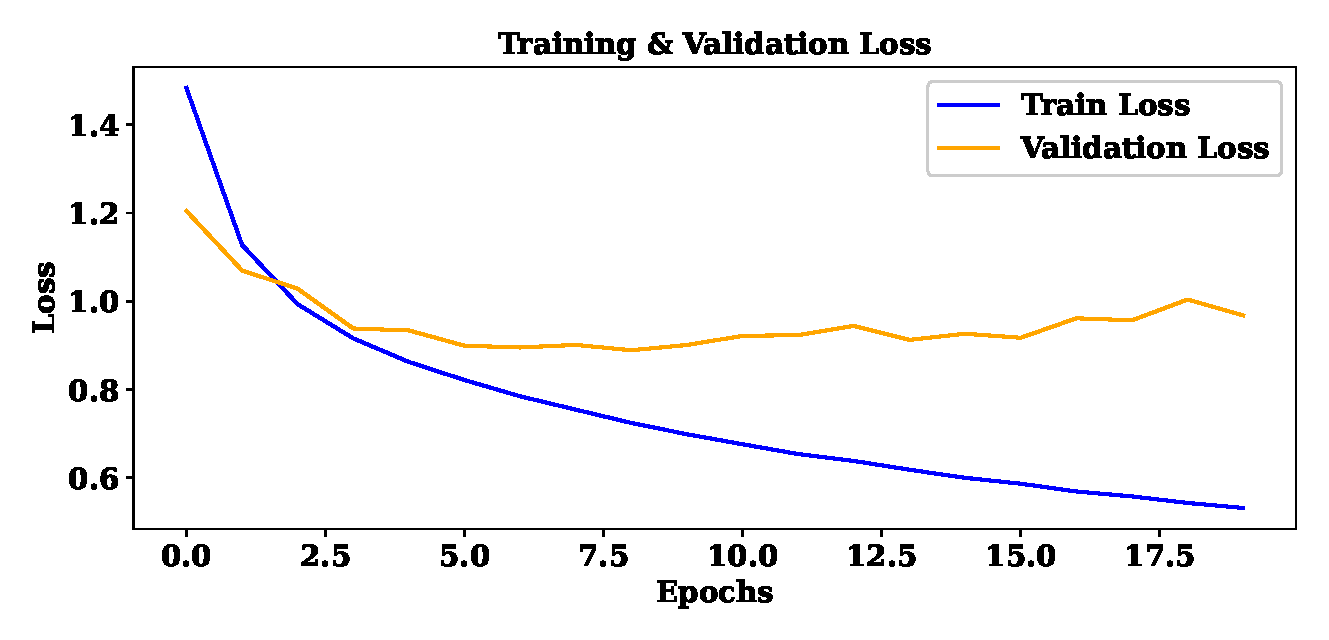
\includegraphics[width=0.85\textwidth]{training_validation_loss.eps}
\caption{Training and validation loss curves over 20 training epochs.}
\label{fig:loss_curves}
\end{figure}
\textbf{Inference:} Training loss continuously decreases toward 0.5, confirming successful optimization gradient steps. Conversely, the validation loss stops improving around epoch 8 and slightly increases up to 1.0, signaling that training beyond 10 epochs yields diminishing generalization returns.

% ==========================================
% 5. Feature Maps
% ==========================================
\subsection{Feature Maps}
\begin{figure}[H]
\centering
\includegraphics[width=0.85\textwidth]{feature_maps.eps}
\caption{Visualization of eight distinct feature maps extracted after the first convolution layer.}
\label{fig:feature_maps}
\end{figure}
\textbf{Inference:} The feature maps reveal that the first convolutional layer acts primarily as a low-level edge and contrast detector. Distinct channels isolate structural elements, such as vertical boundaries, silhouette outlines, or high-intensity background zones, keeping the spatial layout intact.

% ==========================================
% 6. Confusion Matrix
% ==========================================
\subsection{Confusion Matrix}
\begin{figure}[H]
\centering
\includegraphics[width=0.85\textwidth]{confusion_matrix.eps}
\caption{Confusion matrix detailing correct and misclassified predictions across all ten categories.}
\label{fig:confusion_matrix}
\end{figure}
\textbf{Inference:} The dominant diagonal elements reflect strong overall predictive performance, particularly for structured objects like trucks (825) and ships (803). However, notable off-diagonal clusters expose recurring semantic confusion between structurally similar classes, most prominently between cats and dogs (172 misclassifications).

% Begin Section 10
\section{Additional Exercises}
\begin{enumerate}
    \item \textbf{Calculate the output size for a $64\times64$ image using a $5\times5$ kernel with stride 2 and padding 2.}
    
    The spatial dimensions of the feature map after convolution can be computed using the general formula:
    \[
    \text{Output Size} = \left\lfloor \frac{W - K + 2P}{S} \right\rfloor + 1
    \]
    where $W = 64$ (input width/height), $K = 5$ (kernel size), $S = 2$ (stride), and $P = 2$ (padding).
    
    Substituting the given parameters:
    \[
    \text{Output Size} = \left\lfloor \frac{64 - 5 + 2(2)}{2} \right\rfloor + 1 = \left\lfloor \frac{63}{2} \right\rfloor + 1 = 31 + 1 = 32
    \]
    Thus, the output feature map size is \textbf{$32 \times 32$}.

    \item \textbf{Compute the trainable parameters of a convolution layer having 64 filters of size $3\times3$ and an RGB input.}
    
    The number of trainable parameters in a 2D convolutional layer depends on the kernel spatial dimensions, the number of input channels, and the number of filters (including a bias term for each filter):
    \[
    \text{Parameters} = \left( (K_w \times K_h \times C_{\text{in}}) + 1 \right) \times C_{\text{out}}
    \]
    Given:
    \begin{itemize}
        \item Kernel dimensions ($K_w \times K_h$): $3 \times 3$
        \item Input channels ($C_{\text{in}}$): $3$ (RGB)
        \item Number of filters ($C_{\text{out}}$): $64$
    \end{itemize}
    
    \[
    \text{Parameters per Filter} = (3 \times 3 \times 3) + 1 = 28
    \]
    \[
    \text{Total Parameters} = 28 \times 64 = \mathbf{1{,}792}
    \]

    \item \textbf{Compare ReLU and Sigmoid activation functions.}
    
    \begin{table}[H]
    \centering
    \small
    \begin{tabular}{|l|p{5.5cm}|p{5.5cm}|}
    \hline
    \textbf{Property} & \textbf{ReLU} ($f(x) = \max(0, x)$) & \textbf{Sigmoid} ($f(x) = \frac{1}{1 + e^{-x}}$) \\ \hline
    Output Range & $[0, \infty)$ & $(0, 1)$ \\ \hline
    Gradient Behavior & Constant gradient ($1$) for $x > 0$; avoids vanishing gradients in deep networks. & Vanishing gradient problem for very high or low activation values. \\ \hline
    Computation & Extremely fast (simple zero-threshold operation). & Exponential computation required ($e^{-x}$), making it slower. \\ \hline
    Sparsity & True zero outputs for negative inputs create sparse feature activations. & Outputs dense non-zero values continuously. \\ \hline
    \end{tabular}
    \caption{Comparison between ReLU and Sigmoid activation functions.}
    \end{table}

    \item \textbf{Replace Max Pooling with Average Pooling and compare the results.}
    
    \begin{itemize}
        \item \textbf{Max Pooling:} Extracts the maximum value in each pooling window. It serves as a feature detector for sharp edges, textures, and prominent structural patterns while providing spatial invariance and noise suppression.
        \item \textbf{Average Pooling:} Computes the mean value across the pooling window. This results in a smoothing effect that blends feature intensities together. In image classification tasks, this tends to dilute strong localized features with background pixels, often leading to lower test accuracy compared to Max Pooling.
    \end{itemize}

    \item \textbf{Increase the number of convolution filters from 16 to 64 and analyze the effect on accuracy and computation time.}
    
    \begin{itemize}
        \item \textbf{Effect on Accuracy:} Quadrupling the channel capacity allows the model to learn a much richer set of spatial filters (e.g., specialized textures, edge orientations, and complex visual primitives). This generally improves training and test accuracy up to the point where overfitting occurs.
        \item \textbf{Effect on Computation Time:} Memory usage and floating-point operations (FLOPs) scale linearly with channel depth. Increasing filter count from 16 to 64 quadruples the matrix multiplication parameters and forward/backward propagation time per batch.
    \end{itemize}
\end{enumerate}

% Begin Section 11
\section{Results}
The quantitative performance of the constructed convolutional neural network model evaluated on the CIFAR-10 dataset is structured below.

\subsection{Summary Metrics}
\begin{itemize}
    \item \textbf{Training Accuracy:} 81.57\% ($0.8157$)
    \item \textbf{Testing Accuracy:} 69.84\% ($0.6984$)
    \item \textbf{Precision (Macro Avg):} 70.06\% ($0.7006$)
    \item \textbf{Recall (Macro Avg):} 69.84\% ($0.6984$)
    \item \textbf{F1-score (Macro Avg):} 69.84\% ($0.6984$)
    \item \textbf{Number of Parameters:} 60,362 trainable parameters
\end{itemize}

\subsection{Per-Class Performance Breakdown}
To evaluate structural class boundaries and localized classification errors, Table~\ref{tab:class_report} details the precision, recall, and F1-score computed individually for each category.

\begin{table}[H]
\centering
\small
\begin{tabular}{|l|c|c|c|r|}
\hline
\textbf{Class Name} & \textbf{Precision} & \textbf{Recall} & \textbf{F1-Score} & \textbf{Support} \\ \hline
plane  & 0.74 & 0.70 & 0.72 & 1000 \\ \hline
car    & 0.82 & 0.79 & 0.81 & 1000 \\ \hline
bird   & 0.57 & 0.63 & 0.60 & 1000 \\ \hline
cat    & 0.50 & 0.50 & 0.50 & 1000 \\ \hline
deer   & 0.65 & 0.68 & 0.66 & 1000 \\ \hline
dog    & 0.64 & 0.58 & 0.61 & 1000 \\ \hline
frog   & 0.82 & 0.71 & 0.76 & 1000 \\ \hline
horse  & 0.73 & 0.77 & 0.75 & 1000 \\ \hline
ship   & 0.79 & 0.80 & 0.80 & 1000 \\ \hline
truck  & 0.74 & 0.82 & 0.78 & 1000 \\ \hline \hline
\textbf{Macro Avg} & \textbf{0.70} & \textbf{0.70} & \textbf{0.70} & \textbf{10000} \\ \hline
\textbf{Weighted Avg} & \textbf{0.70} & \textbf{0.70} & \textbf{0.70} & \textbf{10000} \\ \hline
\end{tabular}
\caption{Detailed classification report across individual CIFAR-10 test categories.}
\label{tab:class_report}
\end{table}

% Begin Section 12
\section{Discussion}
\begin{enumerate}
    \item \textbf{Why is convolution preferred over fully connected layers for images?}
    
    Convolutional layers exploit \textbf{spatial locality} by processing pixels in local receptive fields rather than treating every input pixel independently. Fully connected layers flatten images into 1D vectors, completely discarding 2D spatial context (such as adjacent pixel relationships) and creating an explosion of parameters. Convolutions preserve structural geometry, translational patterns, and local dependencies while scaling efficiently to high-resolution inputs.

    \item \textbf{How does stride affect the feature map size?}
    
    Stride defines the step size (in pixels) that the sliding filter moves across the input image. Increasing the stride reduces the spatial dimensions (height and width) of the output feature map inversely, as dictated by:
    \[
    \text{Output Size} \propto \frac{1}{\text{Stride}}
    \]
    A stride of 1 processes every overlapping window, preserving fine details, whereas a stride of $S > 1$ downsamples the feature map by skipping spatial locations, effectively reducing spatial resolution and computational complexity.

    \item \textbf{What is the role of padding?}
    
    Padding serves two primary functions in CNNs:
    \begin{itemize}
        \item \textbf{Preserving Spatial Dimensions:} Unpadded convolutions shrink feature maps at every layer, limiting network depth. Applying padding (such as \textit{Same} padding) preserves height and width throughout deep architectures.
        \item \textbf{Preventing Border Information Loss:} Without padding, edge and corner pixels are sampled fewer times than central pixels during sliding operations. Padding ensures equal feature coverage across image boundaries.
    \end{itemize}

    \item \textbf{Why is pooling used?}
    
    Pooling (e.g., Max or Average Pooling) acts as a spatial downsampling step. Key benefits include:
    \begin{itemize}
        \item \textbf{Dimensionality Reduction:} Shrinks feature map dimensions, significantly lowering computational load and parameter counts in subsequent layers.
        \item \textbf{Translation Invariance:} Makes representations robust to minor shifts, distortions, or translations of input features.
        \item \textbf{Receptive Field Expansion:} Increases the effective field of view for deeper layers, allowing them to capture higher-level abstract features.
    \end{itemize}

    \item \textbf{How do feature maps represent image characteristics?}
    
    Feature maps represent activated spatial responses learned by specific convolutional filters:
    \begin{itemize}
        \item \textbf{Early Layers:} Capture low-level, primitive visual attributes such as edges, color gradients, textures, and simple contours.
        \item \textbf{Deeper Layers:} Combine early activations to encode complex, high-level semantic patterns such as shapes, object parts (e.g., eyes, wheels), and complete object class structures.
    \end{itemize}

    \item \textbf{Why do CNNs require fewer parameters than MLPs?}
    
    CNNs dramatically minimize parameter counts through two main design principles:
    \begin{itemize}
        \item \textbf{Parameter Sharing (Weight Reuse):} A single set of kernel weights is swept across the entire input grid, assuming features learned in one region are useful elsewhere. In contrast, an MLP assigns unique weights to every single pixel connection.
        \item \textbf{Sparse Connectivity:} Each output value in a convolution layer is connected only to a small local patch (receptive field) of inputs, unlike MLPs where every input unit connects to every output neuron.
    \end{itemize}
\end{enumerate}

\section{Source Code}
The source code for the Convolutional Neural Network the result with analysis can be found at \url{https://github.com/faultybyte/deep-learning-lab}

% Begin Section 13
\section{References}
\begin{enumerate}
    \item Goodfellow et al., Deep Learning. 
    \item Bishop, Pattern Recognition and Machine Learning. 
    \item Haykin, Neural Networks and Learning Machines. 
    \item TensorFlow Documentation. 
    \item CIFAR-10 Dataset Documentation. 
\end{enumerate}

\end{document}